\documentclass[french,11pt,notitlepage]{report}
\usepackage[utf8]{inputenc}
\usepackage[T1]{fontenc}
\usepackage{lmodern}
\usepackage[a4paper]{geometry}
\usepackage[francais]{babel}
\usepackage{graphicx}
\usepackage{amssymb}
\usepackage{amsmath}
\usepackage{subcaption} 



\begin{document}
	\title{Functional data analysis applied to neurology}
	\author{Clément Bonvoisin, Pierre Ludmann}
	\date{30 juin 2014}
	\maketitle

	\begin{abstract}
  
Il s'agit de segmenter des signaux de marche,
dans le cadre d'une collaboration du CMLA (ENS Cachan) et Cognac-G (Paris V).

On propose donc ici des algorithmes pour détecter des ruptures.
Cela permet en aval aux médecins de mieux étudier les différents régimes de marche.
Un algorithme efficace et rapide semble encore manquer ;
la marche étant souvent abordée sur de longues durées \cite{Was}.

Si la détection d'un unique changement trouve des implémentations reconnues,
on a cherché à généraliser à de multiples ruptures.
Aussi on a changé le paramètre de décision :
on exige un nombre précis de résultats plutôt qu'un seuil de détection.

Malgré de fortes hypothèses de travail,
on obtient des résultats statisfaisants sur des signaux réels et synthétiques
bien que des améliorations restes possibles.

Son utilisation doit faire place à un apprentissage sur les segments de régime obtenus.
	
	\end{abstract}

\phantom{kcahkcah}

\subsection*{Remerciements}



\addcontentsline{toc}{subsection}{Remerciements}



	\tableofcontents



	\chapter{Introduction au problème}
	
	
	
	\section{Motivations}
	
	
		La motivation initiale de ce stage provient de la médecine,
		et plus particulièrement de la neurologie.
		Le projet, piloté par le groupe Cognac-G,
		vise à analyser en détail des signaux physiologiques,
		issus d'une expérience très simple.
		Le protocole expérimental se décline comme suit :
		
		On place sur le patient un ensemble de capteurs :
	\begin{itemize}
		\item sur la tête
		\item sur la ceinture, dans le dos
		\item sur chaque pied
	\end{itemize}	
	
		Ces capteurs sont des centrales inertielles, qui permettent une mesure de l'accélération et de la vitesse angulaire du patient.

		On lance alors l'acquisition :
	\begin{itemize}
		\item pendant quelques secondes, le patient est à l'arrêt
		\item puis, il commence à marcher sur une dizaine de mètres
		\item effectue un demi-tour
		\item et fait une marche retour.
	\end{itemize}
		
	Il s'arrête, et on peut alors arrêter l'acquisition.

	\begin{figure}[!h]
		\hspace{5.6cm}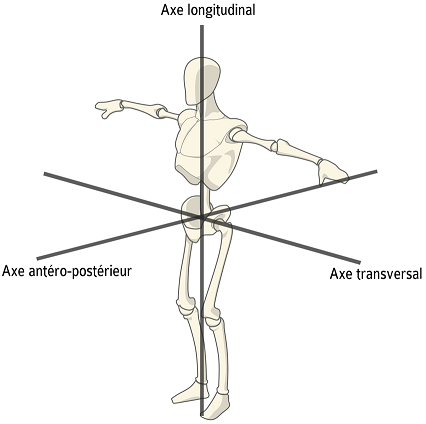
\includegraphics[scale=0.3]{axis.png}
		\caption{Le repère (antéro-postérieur; médio-latéral; vertical)}
		\label{axis}
	\end{figure}
	
	On replace alors les signaux obtenus dans un repère adapté au corps humain, formé de trois axes :
	l'axe antéro-postérieur, l'axe transversal (aussi appelé médio-latéral), et l'axe longitudinal (aussi appelé axe vertical).
		
	\vspace{1pc}
	
	On obtient alors des signaux physiologiques ayant 6 composantes distinctes pour chaque capteur,
	à une fréquence d'acquisition dépendante de la centrale inertielle utilisée ;
	actuellement, le groupe de travail Cognac-G dispose d'instruments permettant un échantillonnage à 100Hz.

% MANQUE DES LABELS
	
	\begin{figure}[!h]
		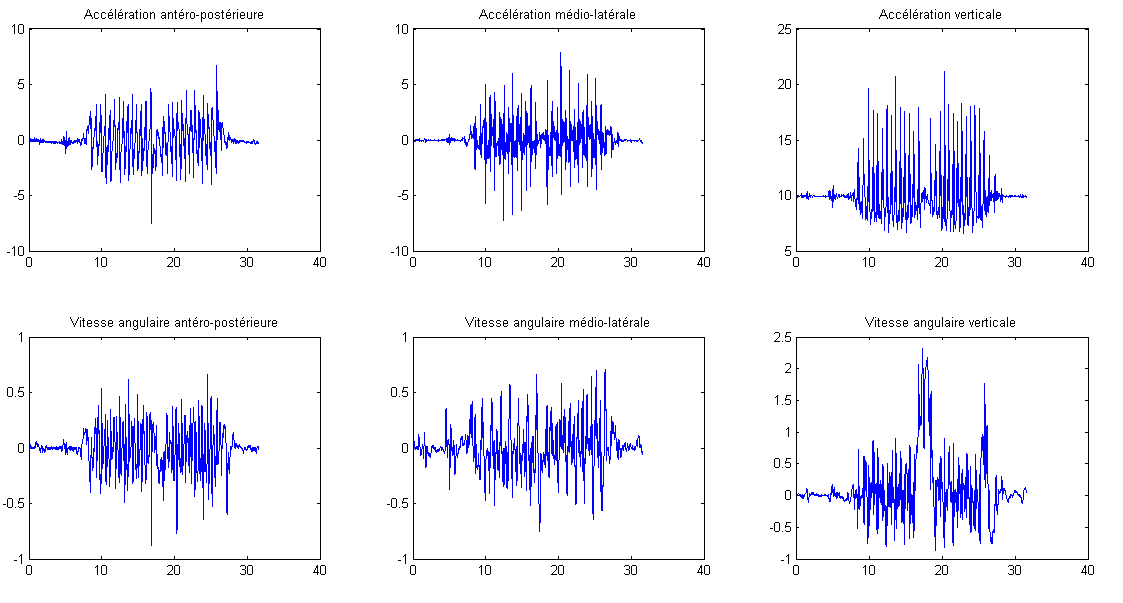
\includegraphics[scale=0.5]{ex_signal_back.png}
		\caption{Un exemple de signal de marche (enregistré à la ceinture)}
		\label{ex_signal_back}
	\end{figure}
	
	Sur ces signaux apparaissent de manière claire les différentes phases de l'expérience :
	\begin{itemize}
		\item Dans un premier temps, le patient est à l'arrêt, les 6 signaux sont quasiment constants (on n'observe que du bruit)
		\item Dans une seconde phase, le patient commence à marcher :
		on peut observer une phase transitoire entre l'arrêt et la marche dite de croisière
		\item La troisième phase de l'expérience correspond à la marche de croisière :
		le patient effectue une dizaine de mètres
		\item On observe ensuite le demi-tour (particulièrement sur les composantes verticales du signal), qui dure environ 1 seconde
		\item Puis, on a une nouvelle phase de marche, retour cette fois-ci
		\item Finalement, le patient s'arrête :
		on a à nouveau une phase transitoire, puis l'arrêt total du patient (où il ne reste plus que du bruit)
	\end{itemize}
	
	\vspace{1pc}
	
	Partant de ces constatations, on peut donc constater que les signaux acquis par les centrales inertielles peuvent être segmentés,
	qu'on peut isoler les différentes phases de l'expérience.
	Sur un signal, cela peut être fait de manière manuelle ;
	néanmoins,
	pour un neurologue enregistrant de manière régulière ce type d'expérience,
	il est concevable de désirer des algorithmes robustes permettant de traiter de manière automatique le problème de la détection des points de changement,
	décomposant ainsi le signal en sous-signaux correspondant à chacune des phases de l'expérience, afin de pouvoir les analyser séparément.
	
	
	\section{Formalisme mathématique}
	
	
	Afin de pouvoir traiter mathématiquement le problème,
	il nous faut tout d'abord poser des définitions claires sur l'objet du problème :
	il s'agit donc de définir ce qu'est une rupture,
	au sens mathématique.
	\\
	
	La littérature propose une approche statistique du problème : 
	on considère les signaux comme la réalisation d'une suite (finie) de variables aléatoires.
%Proposer ici des références bibliographiques...
	\begin{equation}
		(x_i)_{i \in [\![1\,; N]\!]} = (X_i(\omega))_{i \in [\![1\,; N]\!]}
		\label{11}
	\end{equation}
	
	Ce formalisme,
	qui peut paraître quelque peu abstrait en première approche,
	permet d'exprimer de manière simple la notion de rupture dans un signal.
	\\
	
	Sur les signaux précédents, on constate, par exemple,
	une différence nette d'écart-type entre la phase à l'arrêt et la phase de marche ;
	de même, sur la vitesse angulaire verticale, on constate un changement de moyenne entre les phases de marche et le demi-tour.
	Il paraît donc naturel de considérer la distribution statistique des différents points d'un signal multivarié pour formaliser le concept de rupture.
	\\
	
	On comprend alors la définition donnée par la littérature d'un point de rupture à un instant $t_0$ :
	\begin{equation}
	\begin{array}{ll}
			\forall i \in [\![1\,; t_0-1]\!], X_i \sim p_0 \\
			 \forall i \in [\![t_0\,; N]\!], X_i \sim p_1 \\
	\end{array}
	\end{equation}
	%Ref. needed
	
	On généralise de manière évidente au cas de $R$ ruptures aux points $(t_r)_{r \in [\![0\,; n-1]\!]}$ :
	
	\begin{equation}
	\begin{array}{lll}
		~ \forall r \in [\![0\,; R-1]\!], \\
		~ \forall i \in [\![t_{r-1}\,; t_r-1]\!], X_i \sim p_r \\
		( \forall i \in [\![t_r\,; t_{r+1}-1]\!], X_i \sim p_{r+1} )
	\end{array}
	\label{multi_rupt}
	\end{equation}
	
	où l'on a posé : $t_{-1} = 1$ et $t_R = N+1$.
	\\
	
	Ce problème étant formalisé, il s'agit maintenant de trouver des méthodes pour détecter ces points de rupture.
	
	
	
	\chapter{Algorithme CUSUM : résolution du cas d'une seule rupture}
	
	
	
	\section{Principe de l'algorithme CUSUM}
	
	
	L'algorithme CUSUM fut proposé en 1954 par E.S. Page \cite{CIS} ; une methode "en ligne".
	Les signaux étant ici déjà réalisés, il nous faut ici adapter l'algorithme au cas "hors ligne" \cite{DAC}.
	\\
	
	Dans le formalisme précédent, on conçoit que les méthodes de détection de rupture se fondent sur des outils statistiques.
	L'idée de base de l'algorithme CUSUM hors ligne est la suivante :
	comparer l'hypothèse qu'il existe une rupture dans le signal considéré à l'hypothèse qu'il n'y en a pas.
	L'outil utilisé pour cette comparaison est la notion de vraisemblance.
	Pour simplifier, on fera maintenant l'hypothèse d'indépendance des variables aléatoires $(X_i)_{i \in [\![1\,; N]\!]}$.
	\\
	
	La fonction de vraisemblance quantifie la vraisemblance d'une hypothèse étant donnée une observation.
	Ici, l'observation faite est le signal, qui est la réalisation d'un nombre fini de variables aléatoires.
	On cherche à comparer l'hypothèse $H_t$ qu'à l'instant $t$, il y a une rupture, à l'hypothèse $H_0$ qu'il n'y en a pas dans le signal.
	Les vraisemblances de ces hypothèses sont :
	\begin{equation}
	\begin{array}{ll}
		\forall t \in [\![1\,; N]\!], l(H_t) = \prod_{i = 1}^{t-1} p_0(x_i) \prod_{i = t}^{N} p_1(x_i) \\\\
		\phantom{\forall t \in [\![1\,; N]\!], }l(H_0) = \prod_{i = 1}^N\tilde p(x_i) \\
	\end{array}	
	\end{equation}
	
	Introduisons alors le rapport de vraisemblance des hypothèses :
	\begin{equation}
		\forall t \in [\![1\,; N]\!], \Lambda_t = \frac{l(H_t)}{l(H_0)} = \frac{\prod_{i = 1}^{t-1} p_0(x_i) \prod_{i = t}^{N} p_1(x_i)}{\prod_{i = 1]}^{N} \tilde p(x_i)}
	\end{equation}
	
	Pour simplifier, on fera ici l'hypothèse que nos lois sont issues d'une famille de lois indexée par un paramètre $\theta$ qui vit dans un espace donné.

	On a ainsi :
	
	\begin{equation*}
		p_0 = p_{\theta_0}~;~p_1 = p_{\theta_1}~;~\tilde p = p_{\tilde\theta}
	\end{equation*}
	
	On ne connaît pas, a priori, les paramètres $\tilde\theta$, $\theta_0$ et $\theta_1$.
	Pour les estimer, on va donc utiliser l'estimation du maximum de vraisemblance.
	Il en découle alors la formule suivante, à la base de l'algorithme CUSUM, qui donne le logarithme du rapport de vraisemblance (\textit{log-likelihood ratio}, en anglais) :
	
	\begin{equation}
		\forall t \in [\![1\,; N]\!], L_t=\ln \left[ \frac{\sup_{\theta_0}\left\{ \prod_{i=1}^{k-1} p_{\theta_0}(x_i) \right\} \cdot \sup_{\theta_0} \left\{ \prod_{i = k}^{N}p_{\theta_0}(x_i) \right\}}{\sup_{\tilde\theta}\left\{\prod_{i=i}^{N}p_{\tilde{\theta}}(x_i)\right\}} \right]
		\label{log_likelihood_ratio}
	\end{equation}
	
	Finalement, l'instant où il est le plus probable de trouver une rupture est celui qui maximise $L_t$.
	Ainsi, l'estimation de maximum de vraissemblance (\emph{maximum likelihood estimation}) par CUSUM du point de rupture d'un signal est :
	
	\begin{equation}
		\hat{t_0}=\arg\max_{1\le t\le N}L_t
	\end{equation}
	
	
	\section{Simplification dans le cas de distributions gaussiennes}

	
	Dans le cas général, la formule \ref{log_likelihood_ratio} est peu exploitable en raison de la présence de bornes supérieures.
	Afin de simplifier le problème des estimateurs au maximum de vraisemblance
	, on peut se proposer de faire une hypothèse sur la famille de lois $(p_\theta)_{\theta \in \mathbb{R}^d}$.
	\\
	
	On suppose donc, à partir de maintenant, que chacune des variables aléatoires qui composent le signal suit une loi gaussienne, \emph{i.e.} :
	
	\begin{equation*}
		p_{\mu, \sigma}(y) = \frac1{\sigma\sqrt{2 \pi}} \exp \left[ -\frac12 \left( \frac{y - \mu}{\sigma} \right)^2 \right]
	\end{equation*}
	
	Les estimateurs aux maximas de vraisemblance de la loi normale sont alors connus \cite{MLE}.
	Ceci nous permet alors de simplifier l'expression de $L_t$
	car les bornes supérieures sont atteintes par ces estimateurs.
	Notons que l'hypothèse du gaussien ramène le problème du changement de loi à trois cas :
	changement de moyenne, changement d'écart-type, et changement de moyenne et d'écart-type.
	
		Bien que nous n'allons pas immédiatement traîter les signaux physiologiques vus précédemment --
	ceux-ci comportent plusieurs ruptures, l'algorithme CUSUM ne permettant d'en détecter qu'une seule -- il est de bon ton de joindre des exemples imagés à ce flot de formules.
	Les signaux utilisés dans cette partie sont des signaux synthétiques, obtenus grâce à MATLAB.
	
		Aussi les détails et preuves de cette simplification se trouvent en annexe.
		
	
	\subsection{Changement en moyenne}
	
	
	Faisant l'hypothèse d'un écart-type constant sur l'ensemble du signal, le paramètre $\theta$ est ici uniquement la moyenne $\mu$.
	
	\ref{log_likelihood_ratio} se réécrit donc après calculs :
	\begin{equation}
		\forall t \in [\![1\,; N]\!], L_t = \frac{1}{2 \sigma ^2}\left[(t-1){\mu_0}^2 + (N - t + 1){\mu_1}^2 - N{\tilde\mu}^2 \right]
		\label{meanchange}
	\end{equation}
	
	$\sigma$ étant donc fixé au préalable. Et $\tilde\mu$, $\mu_0$ et $\mu_1$ sont les estimateurs $\frac1n\sum_{i=1}^nx_i$ du signal respectivement de 1 à $N$, de 1 à $t-1$ et de $t$ à $N$.
	\\
	
	On se place dans le cas d'un changement en moyenne de $\mu_1 = 10$ à $\mu_2 = 20$, avec $t_0 = 201$.
	
	On utilise cette fois l'équation \ref{meanchange} pour obtenir la figure \ref{llr_test_mean}.


	\begin{figure}[h]	
		\begin{subfigure}[t]{.49\textwidth}

  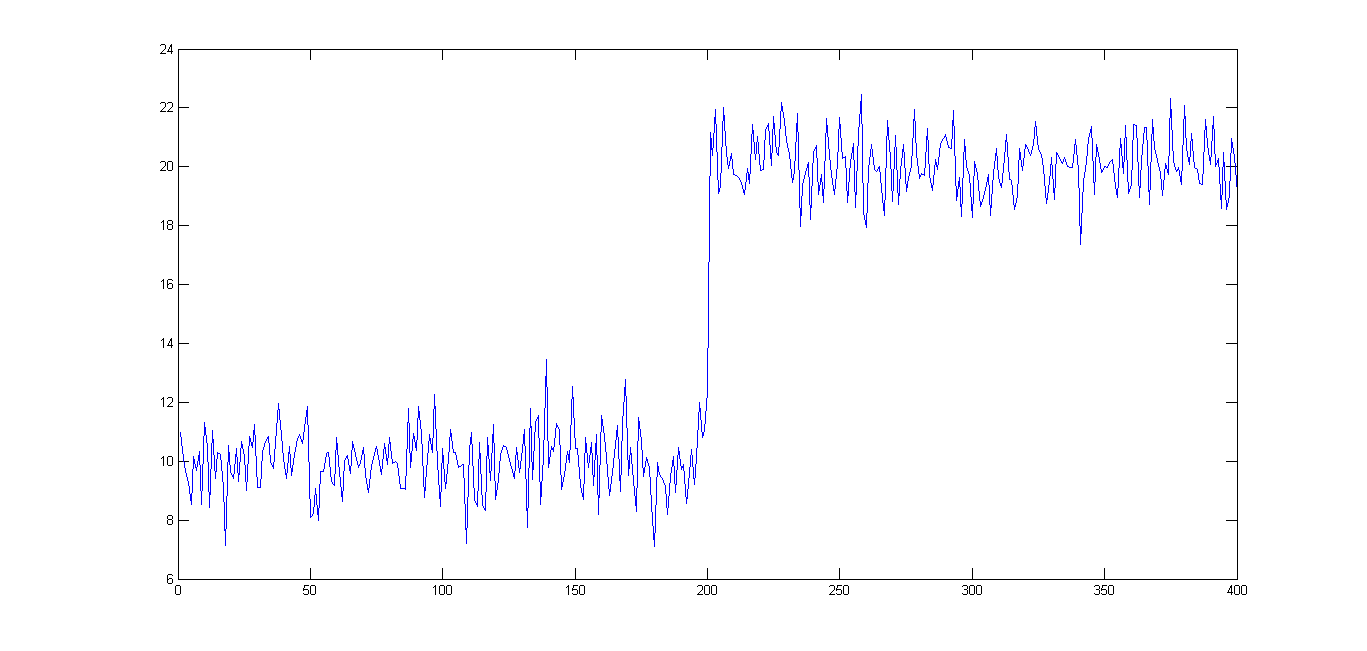
\includegraphics[width=\linewidth]{test_signal_mean.png}
		\caption{Pour $t \leq 200$, $X_t \sim \mathcal{N}(10, 1)$ ; pour $t > 200$, $X_t \sim \mathcal{N}(20, 1)$}
		\label{test_signal_mean}
	\end{subfigure}
	\hfill
	\begin{subfigure}[t]{.49\textwidth}

  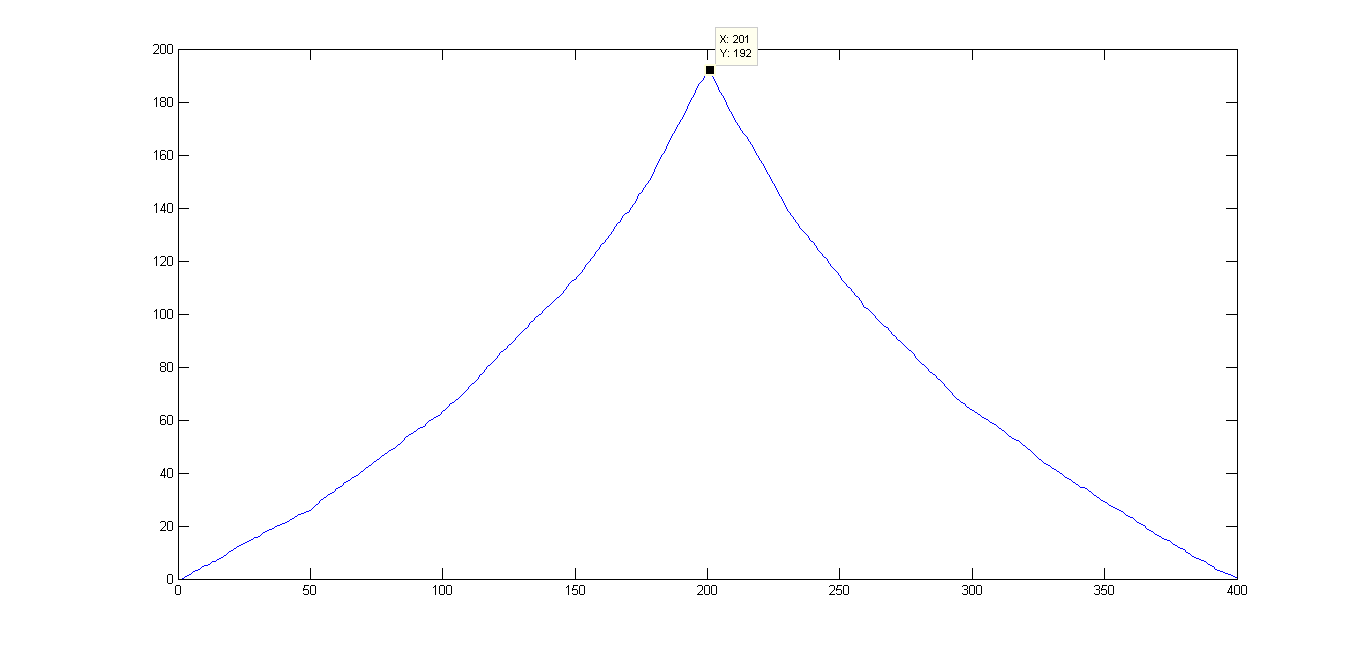
\includegraphics[width=\linewidth]{llr_test_mean.png}
		\caption{\textit{Log-likelihood ratio} du signal précédent}
		\label{llr_test_mean}
	\end{subfigure}
	
	\caption{Exemple de détection d'une rupture par la moyenne}
	\end{figure}
	
	On obtient donc ici l'estimateur du point de rupture par CUSUM, avec un score de 192 :
	\begin{equation*}
		\hat{t_0} = 201 ; \hat{t_0} - t_0 = 0
	\end{equation*}
	
	De même que dans le cas précédent, on observe la robustesse de l'estimateur par CUSUM du point de rupture de ce signal. Pour quantifier cette robustesse, on peut s'appuyer sur la déviation quadratique moyenne de cet estimateur (RMSD), en répétant 5.000 fois l'expérience précédente, on trouve : $RMSD = 0$.
	
	
	\subsection{Changement en écart-type}
	
	
	Faisant cette fois l'hypothèse d'une moyenne constante sur l'ensemble du signal, le paramètre $\theta$ est ici uniquement l'écart-type $\sigma$.
	
	\ref{log_likelihood_ratio} se réécrit alors : 
	
	\begin{equation}
		\forall t \in [\![1\,; N]\!], L_t = N\ln (\tilde{\sigma}) - (t-1)\ln ({\sigma_0}) - (N-t+1)\ln ({\sigma_1})
		\label{stdchange}
	\end{equation}
	$\mu$ étant préalablement fixé. Et $\tilde\sigma$, $\sigma_0$ et $\sigma_1$ sont les estimateurs $\sqrt{\frac1n\sum_{i=1}^n(x_i-\mu)^2}$ du signal respectivement de 1 à $N$, de 1 à $t-1$ et de $t$ à $N$.
	\\
	
		On se place dans le cas d'un changement en écart-type de $\sigma_0 = 1$ à $\sigma_1 = 3$, à l'instant $t_0 = 201$.
	

	
	\begin{figure}[h]

	\begin{subfigure}[t]{.49\textwidth}

  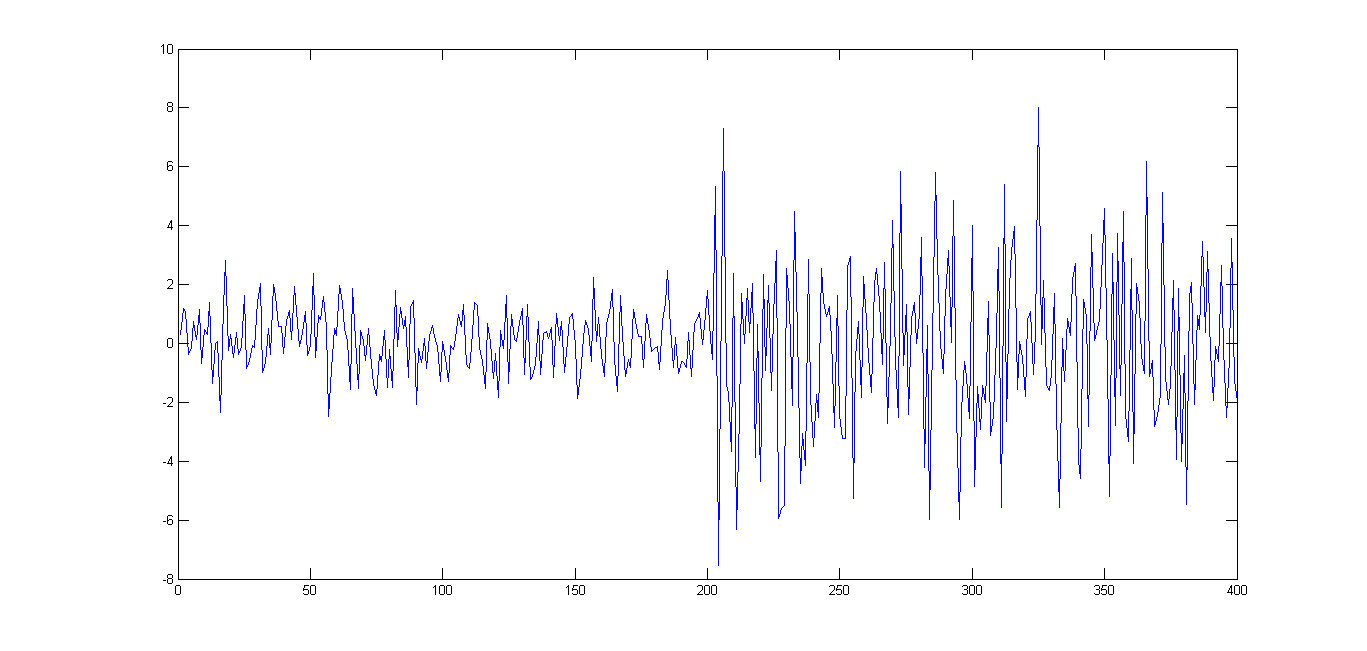
\includegraphics[width=\linewidth]{test_signal_std.png}
		\caption{Pour $t \leq 200$, $X_t \sim \mathcal{N}(0, 1)$ ; pour $t > 200$, $X_t \sim \mathcal{N}(0, 3)$}
		\label{test_signal_std}
	\end{subfigure}
	\hfill
	\begin{subfigure}[t]{.49\textwidth}

  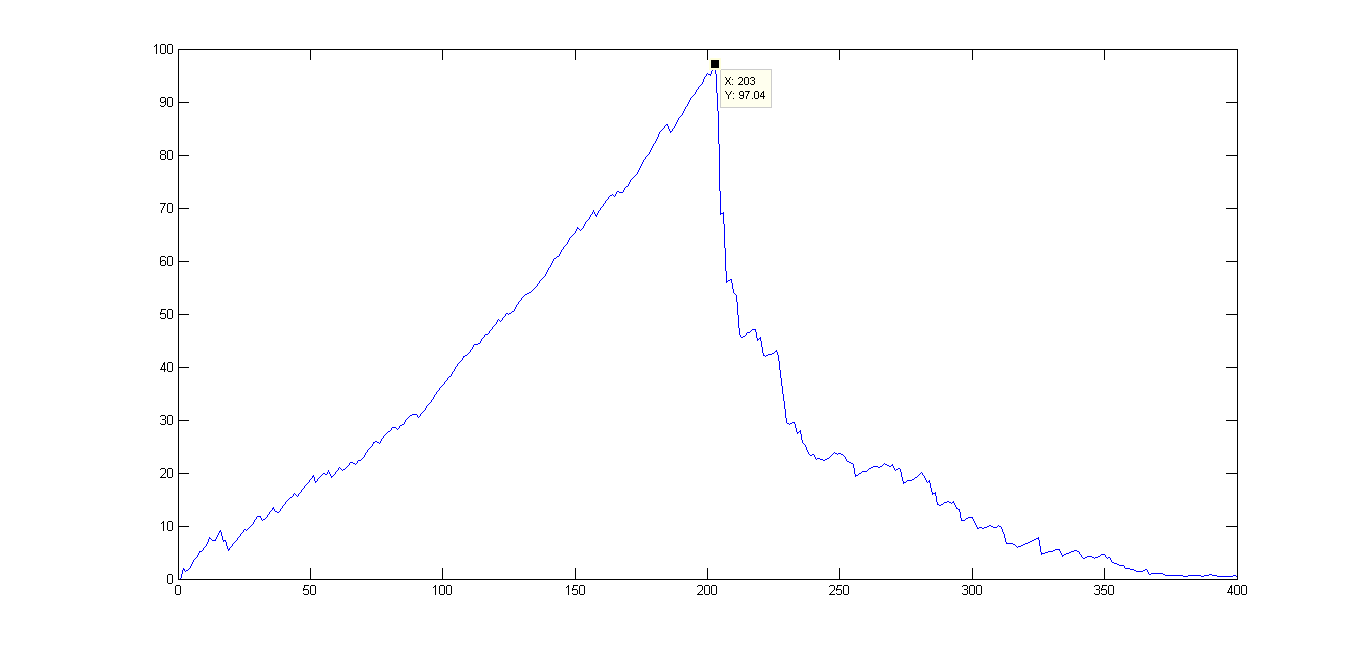
\includegraphics[width=\linewidth]{llr_test_std.png}
		\caption{\textit{Log-likelihood ratio} du signal précédent}
		\label{llr_test_std}
	\end{subfigure}
	\caption{Exemple de détection d'une rupture par l'écart-type}
	\end{figure}
	

	
	L'équation \ref{stdchange} permet alors d'obtenir la figure \ref{llr_test_std}
		
	Ce comportement est le comportement typique de la courbe d'un \textit{log-likelihood ratio} sur un signal gaussien comportant une rupture. On observe ici que le maximum de la courbe est à l'instant 203, avec un \textit{log-likelihood ratio} $L_{203} = 97,04$. On a donc l'estimateur par CUSUM du point de rupture :
	\begin{equation*}
		\hat{t_0} = 203 ; \hat{t_0} - t_0 = 2;
	\end{equation*}
	
	Ainsi, l'estimateur de points de rupture par CUSUM semble robuste dans le cas d'un changement par écart-type. Pour 5.000 signaux différents suivant les caractéristiques précédentes, on trouve : $RMSD = 2,605$.
	
	
	\subsection{Changement en moyenne et en écart-type}
	
	
	Dans ce dernier cas, on doit estimer à la fois la moyenne et l'écart-type des différentes portions du signal. On obtient un résultat quasiment identique à \ref{stdchange} :
	\begin{equation}
		\forall t \in [\![1\,;N]\!], L_t = N\ln (\tilde\sigma) - (t-1) \ln (\sigma_0) - (N - t + 1) \ln (\sigma_1)
		\label{bothchange}
	\end{equation}
	La seule différence intervient dans l'estimateur de l'écart-type :
	au lieu d'utiliser une moyenne fixée sur l'ensemble du signal (ce qui peut se traduire légitimement par son estimateur sur la globalité du signal),
	on utilise ici les estimateurs  de la moyenne sur les différentes portions du signal :
	
	$\tilde\mu$, $\mu_0$ et $\mu_1$ sont les estimateurs $\frac1n\sum_{i=1}^nx_i$ du signal respectivement de 1 à $N$, de 1 à $t-1$ et de $t$ à $N$.
	Et $\tilde\sigma$, $\sigma_0$ et $\sigma_1$ sont les estimateurs $\sqrt{\frac1n\left[\sum_{i=1}^nx_i^2-(\sum_{i=1}^nx_i)^2\right]}$ du signal respectivement de 1 à $N$, de 1 à $t-1$ et de $t$ à $N$.
	
	\subsection{Détection d'un changement de moyenne}
	
	

	
	
	
	\chapter{Cas de plusieurs ruptures : implémentation dichotomique}



	Nous avons déjà présenté, dans le premier chapitre, le formalisme statistique associé au cas de plusieurs ruptures dans un signa (cf. équation \ref{multi_rupt}).
	
	
	
	\chapter{Cas de plusieurs ruptures : implémentation par fenêtres}
	
	
	
	
	
	
	\chapter{Évaluation des performances}
	
	
	
	
	
	
	\chapter{Conclusion}
	
	
	
\bibliographystyle{alpha}
\bibliography{Rapport.bib}
	
\end{document}
